\documentclass[11pt, a4paper]{article}
\usepackage[letterpaper, portrait, margin=0.5in]{geometry}
\usepackage[english]{babel}  % force American English hyphenation patterns
\usepackage{amsmath,mathtools}

\usepackage{graphicx}
\usepackage{wrapfig}


\begin{document}
\title{Chapter 16 Sound Waves}
\author{Apostolos Delis}
\date{\today}
\maketitle

\tableofcontents
\section[16.1, Sound Waves]{Sound Waves}
\begin{itemize}
    \item The simplest sound waves are sinusoidal waves, which have definite frequency,
        amplitude, and wavelength.
    \item  If the wave is sinusoidal going in the +x direction, we can express it by
        using:
        \begin{equation}
            y(x,t) = A\cos(kx -\omega t)
        \end{equation}
\end{itemize}
\subsection{Perception of sound Waves}
\begin{itemize}
    \item For a given frequency, the greater the pressure amplitude of a sinusoidal
        sound wave, the greater the perceived loudness
    \item The frequency of a sound wave is the primary factor in determining the pitch of
        a sound
    \item Unlike the tones made by musical instruments, noise is a combination of all
        frequencies, not just frequencies that are integer multiples of a fundamental
        frequency
\end{itemize}
\section[16.2, Speed of Sound Waves]{Speed of Sound Waves}
\begin{itemize}
    \item Earlier we found that the speed $v$ of a transverse wave on a string depends on
        the string tension $F$ and the linear mass density $\mu$: $v =$
        $\sqrt{\frac{F}{\mu}}$, we may want to ask, on what properties of the medium does
        the speed depend?
    \item For mechanical waves, the speed of the wave is of the form:
        \begin{equation}
            v = \sqrt{\frac{\text{Restoring force returning the system equilibrium}}
            {\text{Inertia resisting the return to equilibrium}}}
        \end{equation}
    \item According to Newton’s second law, inertia is related to mass. We can describe
        this with the mass per unit volume $\rho$, so speed of sound waves should be of
        the form $v = \sqrt{\frac{B}{\rho}}$
\end{itemize}
\section[16.3, Sound Intensity]{Sound Intensity}
\begin{itemize}
    \item Consider a sound wave propagating in the $+x$ direction, so we can use the
        expression found for $y(x,t)$ in Section 16.1
    \item Note that power per unit area in this sound wave equals the product of
        $p(x,t)$, and the particle velocity, $v_y(x,t)$, which is the velocity at time
        $t$ of that portion of the wave medium. We find that
        \begin{equation}
            v_y(x,t) = \frac{\partial y(x,t)}{\partial t} = \omega A\sin(kx - \omega t)
        \end{equation}
        And that leads to
        \begin{equation}
            p(x,t)v_y(x,t) = [BkA\sin(kx - \omega t)][\omega A\sin(kx - \omega t)] =
            B\omega kA^{2}\sin^{2}(kx - \omega t)
        \end{equation}
    \item The intensity is the time average value of the power unit area
        $p(x,t)v_y(x,t)$. For any value $x$, the average value of $\sin^2(kx - \omega t)$
        over one period $T = \frac{2\pi}{\omega}$ is $\frac{1}{2}$ so
        \begin{equation}
            I = \frac{1}{2}B\omega kA^2
        \end{equation}
        Where here $\rho$ is the density of the fluid, $B$ is the bulk modulus of the
        fluid, and $\omega = 2\pi f$
\end{itemize}
\subsection{The decibel scale}
\begin{itemize}
    \item Because the ear is sensitive over a broad range of intensities, a logarithmic
        measure of intensity called sound intensity level is often used
        \begin{equation}
            \beta = (10 dB)\log \frac{I}{I_0}
        \end{equation}
        Where $I_0 = 10^{-12} W / m^2$ is the reference intensity
    \item Using the decibel scale, $\beta = 0$ corresponds to $I = I_0$ and a $I = 1W /$
        $m^2$ corresponds to $\beta = 120$
        corresponds
    \item This scale deemphasizes the low and very high frequencies, where the ear is
        less sensitive
\end{itemize}
\section[16.8, The Doppler Effect]{The Doppler Effect}
\begin{itemize}
   \item When a car approaches you with its horn sounding, the pitch seems to drop as
       the car passes; the phenomena is known as the Doppler Effect
   \item Let $v_s$ and $v_L$ be the direction from the listener $L$ to the source $S$.
       The speed of sound relative to the medium, $v$ is always considered positive
\end{itemize}
\subsection{Moving Listener And Stationary Source}
\begin{itemize}
    \item Think about a Listener L moving with velocity $v_L$ toward a stationary source
        $S$. The source emits a sound wave with frequency $f_S$ and a wavelength
        $\lambda = \frac{v}{f_S}$
    \item The Wave crests approaching the moving listener have a speed of propagation
        $relative$ to the $listener$ of $(v+v_L)$. So the frequency $f_L$ with which the
        crests arrive at the listener's position is
        \begin{equation}
            f_L = \frac{v+v_L}{\lambda} = \frac{v+v_L}{v / f_S}
        \end{equation}
        This can then be written as
        \begin{equation}
            f_L = \bigg(\frac{v+v_L}{v}\bigg)f_S = \bigg(1 + \frac{v_L}{v}\bigg)f_S
        \end{equation}
        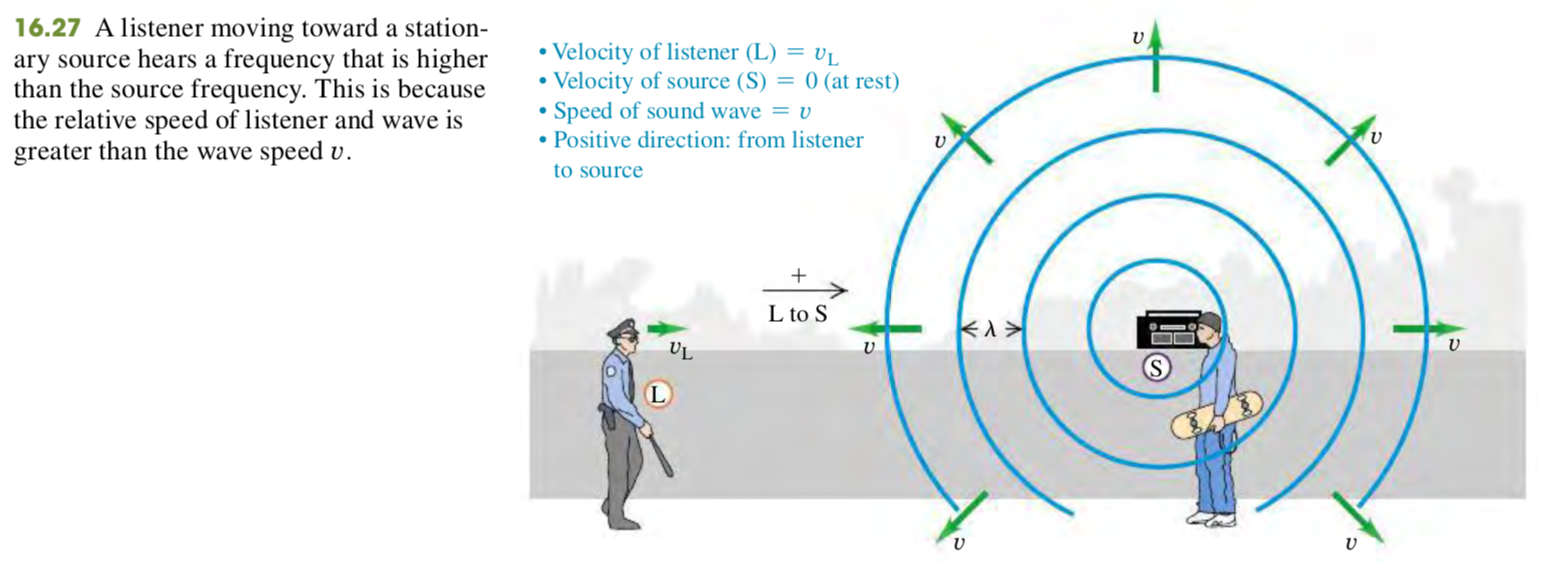
\includegraphics[scale=0.65]{images/doppler_effect.png}
\end{itemize}
\subsection{Moving source and Moving Listener}
\begin{itemize}
    \item Now suppose the source is moving as well, with a velocity $v_S$, The wave speed
        is still $v$, but the wavelength is no longer $v / f_S$.
    \item To find the frequency heard by the listener behind the source, we substitute
        the equation
        \begin{equation}
            \lambda_{behind} = \frac{v + v_S}{f_S}
        \end{equation}
        into the equation
        \begin{equation}
            f_L = \frac{v+v_L}{\lambda_{behind}} = \frac{v+v_L}{v+v_S}f_S
        \end{equation}
\end{itemize}
\end{document}

